chapter{On ws-Homeomorphism in Topological Space}
\ifpdf
\graphicspath{{Chapter2/Chapter2Figs/}}
\else
\graphicspath{{Chapter2/Chapter2Figs/EPS/}{Chapter2/Chapter2Figs/}}
\fi

\parindent 0.75cm
\parskip 0.25cm

\newtheorem{theorem}{Theorem}[section]
\theoremstyle{plain}
\newtheorem{acknowledgement}{Acknowledgement}
\newtheorem{algorithm}{Algorithm}[section]
\newtheorem{axiom}{Axiom}[section]
\newtheorem{case}{Case}[section]
\newtheorem{claim}{Claim}[section]
\newtheorem{conclusion}{Conclusion}[section]
\newtheorem{condition}{Condition}[section]
\newtheorem{conjecture}{Conjecture}[section]
\newtheorem{corollary}[theorem]{Corollary}
\newtheorem{criterion}{Criterion}[section]
\newtheorem{definition}{Definition}[section]
\newtheorem{example}{Example}[section]
\newtheorem{exercise}{Exercise}[section]
\newtheorem{lemma}{Lemma}[section]
\newtheorem{notation}{Notation}[section]
\newtheorem{problem}{Problem}[section]
\newtheorem{proposition}{Proposition}[section]
\newtheorem{remark}[theorem]{Remark}
\newtheorem{solution}{Solution}[section]
\newtheorem{summary}{Summary}[section]
\numberwithin{equation}{section}
\def\baselinestretch{1.5}
\section{intoduction}
The concept of generalized homeomorphism was derived and studied in the year 1991 by Maki et all [5]. N. Nagaveni [25] introduced and investigated rwg homeomorphism in topological space. In the year 2002, M Sheik John [30] introduced and investigated w- homeomorphism in topological space. The intention of the paper is to analyze and study ws-homeomorphism, ws*-homeomorphism and their relation with some existing homeomorphisms in topological space. Also some of their properties have been verified.
In second of this chapter, we to introduce and study ws-homeomorphism, ws*-homeomorphism and their relation with some existing homeomorphisms in topological space. Also some of their properties have been investigated
\section{ws-Homeomorphism in Topological Space}
\begin{Definition} A bijective map h: (P,τ)→(Q,σ) is termed as ws-homeomorphism if h is both ws-continuous and ws-open.
\end{Definition}
\begin{example}
	 Take up P=Q=\\{1,2,3}, τ =\{P, ϕ,\{1},\{2},\{1,2}}be a topology on P and σ =\{Q, ϕ,\{1},\{2},\{1,2},\{1,3}} be a topology on Q and wsC(P)= \{φ, P, \{1}, \{2},\{3}, \{1, 3},\{2, 3}}
And wsO(Q) =\{Q, ϕ,\{1},\{2},\{1,2},\{1,3}}.Take up  h: P→Q defined by identity map then h is ws–homeomorphism
\end{example}
\begin{theorem}
	 Each homeomorphism is a ws-homeomorphism but inverse is untrue.
\end{theorem}
\begin{Proof} Take up h: P→Q be a homeomorphism. Then h is bijective, continuous and open map. Since each continuous map is ws-continuous and each open map is ws-open, h is ws-homeomorphism.
Example 5.2.4: Take up P=Q= \{1, 2, 3}. Let τ= \{  ,P, \{1}, \{2},\{1,2}}be a topology on P and σ=\{, Q, \{1}, \{2}, \{1, 2}, \{1 3}} be a topology on Q and  wsC(P)= \{φ, P, \{1}, \{2},\{3}, \{1, 3},\{2, 3}}. Let h: (P,  τ )→(Q, σ) be a function defined by identity map is ws- homeomorphism but not a homeomorphism as the closed set  H=\{2} in Q, h^(-1)(H)=\{2} is not a closed  in P hence not a continuous function therefore not a homeomorphism.
\end{Proof}
\begin{theorem}
	If a map h: P→Q is homeomorphism then the following holds.
\end{theorem}

%
Hand-drawn figures, downloaded/created images \& graphs need to be inserted in a document. There are different ways to insert these in a document. 


\section{Insert an image}

One image as in Figure \ref{Fig21} is to be inserted. Looks good if it is located in the center. The size can be adjusted to suit the needs. 

\begin{figure}[!htbp]
	\begin{center}
		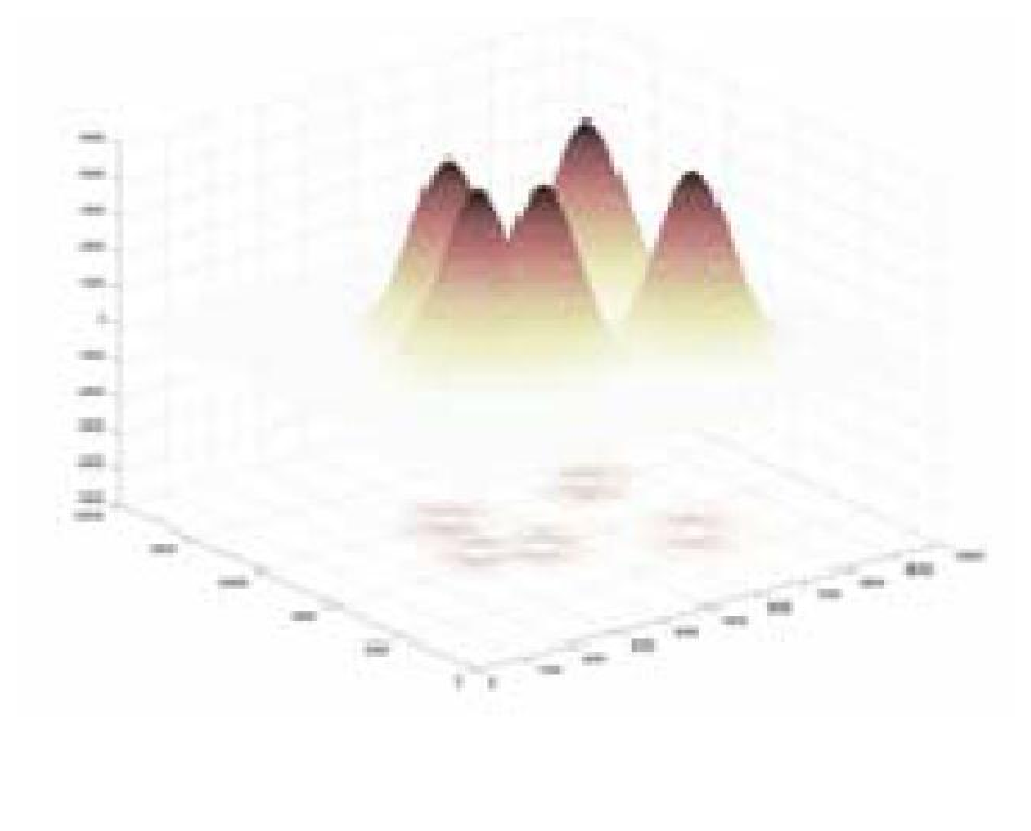
\includegraphics [scale=0.5]{small_width}
		\caption{Gaussian kernel}
		\label{Fig21}
	\end{center}
\end{figure}

\chapter{Tabular environment}
\graphicspath{{Chapter4/Chapter4Figs/EPS/}{Chapter4/Chapter4Figs/}}

%
Information in the form of a matrix or table is created using the tabular environment. The following sections give you ways to create tables. 

\section{Simple table}

Table \ref{Tab1} has two columns and a few rows. Values in each column can be left-aligned, right-aligned or centered. Sequence of rows are created using $\backslash\backslash$ commands. Each row is a sequence of items separated by \& character. $\backslash$hline is used to draw horizontal lines whereas $|$ draws vertical lines in the entire environment. 

\begin{table}
\caption{\label{Tab1}Simple table}
\begin{center}
\begin{tabular}{|l|r|} \hline
Parameter         & Value      \\ \hline \hline
$\alpha$          & 0.9        \\ \hline
$\beta$           & 100        \\ \hline
$\gamma$          & 0.5        \\ \hline
$\eta$            & 0.1        \\ \hline
\end{tabular}
\end{center}
\end{table}

\section{Table with more formatting}

Table \ref{Tab2} has some additional features for formatting. It incorporates the multirow and multicolumn features. 

\begin{table}
\caption{\label{Tab2}Table with more formatting features}
\begin{center}
\begin{tabular}{|c|c|r|r|r|r|}\hline 
\multirow{2}{*}{Sl. No} &\multirow{2}{*}{Parameter} 
&\multicolumn{4}{c|}{Output Values}\\ \cline{3-6} 
& &Case 1 &Case 2 &Case 3 &Case 4 \\ \hline \hline
\multirow{4}{*}{1} & A & 21 & 19 & 16 & 14  \\
                   & B & 25 & 18 & 16 & 12  \\
                   & C & 47 & 26 & 14 & 10  \\
                   & D & 16 & 14 & 13 & 10  \\ \hline
\multirow{4}{*}{2} & A & 15 & 15 & 14 & 13  \\
                   & B & 18 & 17 & 16 & 16  \\
                   & C & 66 & 41 & 28 & 19  \\
                   & D & 15 & 14 & 14 & 13  \\ \hline
\end{tabular}
\end{center}
\end{table}

%------------------------------------------------------------------------- 
